\documentclass[a4paper,12pt]{article}
\usepackage{amssymb}
\usepackage{amsmath}
\usepackage[utf8]{inputenc}
\usepackage[german]{babel}
\usepackage[T1]{fontenc}
\usepackage[margin=2.5cm]{geometry}
\usepackage{booktabs}
\usepackage{pdfpages}

\usepackage{hyperref}

\makeglossary 

\newcommand{\authorName}{Hendrik Lüth}
\newcommand{\Arbeitgeber}{Ausbildungswerkstatt der Marine}
\newcommand{\projekt}{DDS-Signalgenerator}
\title{\projekt \\ Lastenheft Gehäuse}
\author{\authorName\\ \Arbeitgeber }

\begin{document}
\pagenumbering{roman}
\maketitle
\setcounter{page}{2}
\tableofcontents
\clearpage
\pagenumbering{arabic}

\section{Auftrag}
Es ist ein Gehäuse für den Signalgenerator herzustellen. Als Gehäuse wird ein Plastik-Gehäuse benutzt werden, welches bei dem Lieferanten Reichelt Elektronik\footnote{https://www.reichelt.de/} unter der Bestellnummer \glqq GEH KS 21\grqq\ zu bestellen ist. Der Gehäuseplan liegt diesem Lastenheft bei. Ebenfalls liegt eine Zeichnung mit den nötigen Modifikationen bei.

\section{Gehäuseplan}
\begin{center}
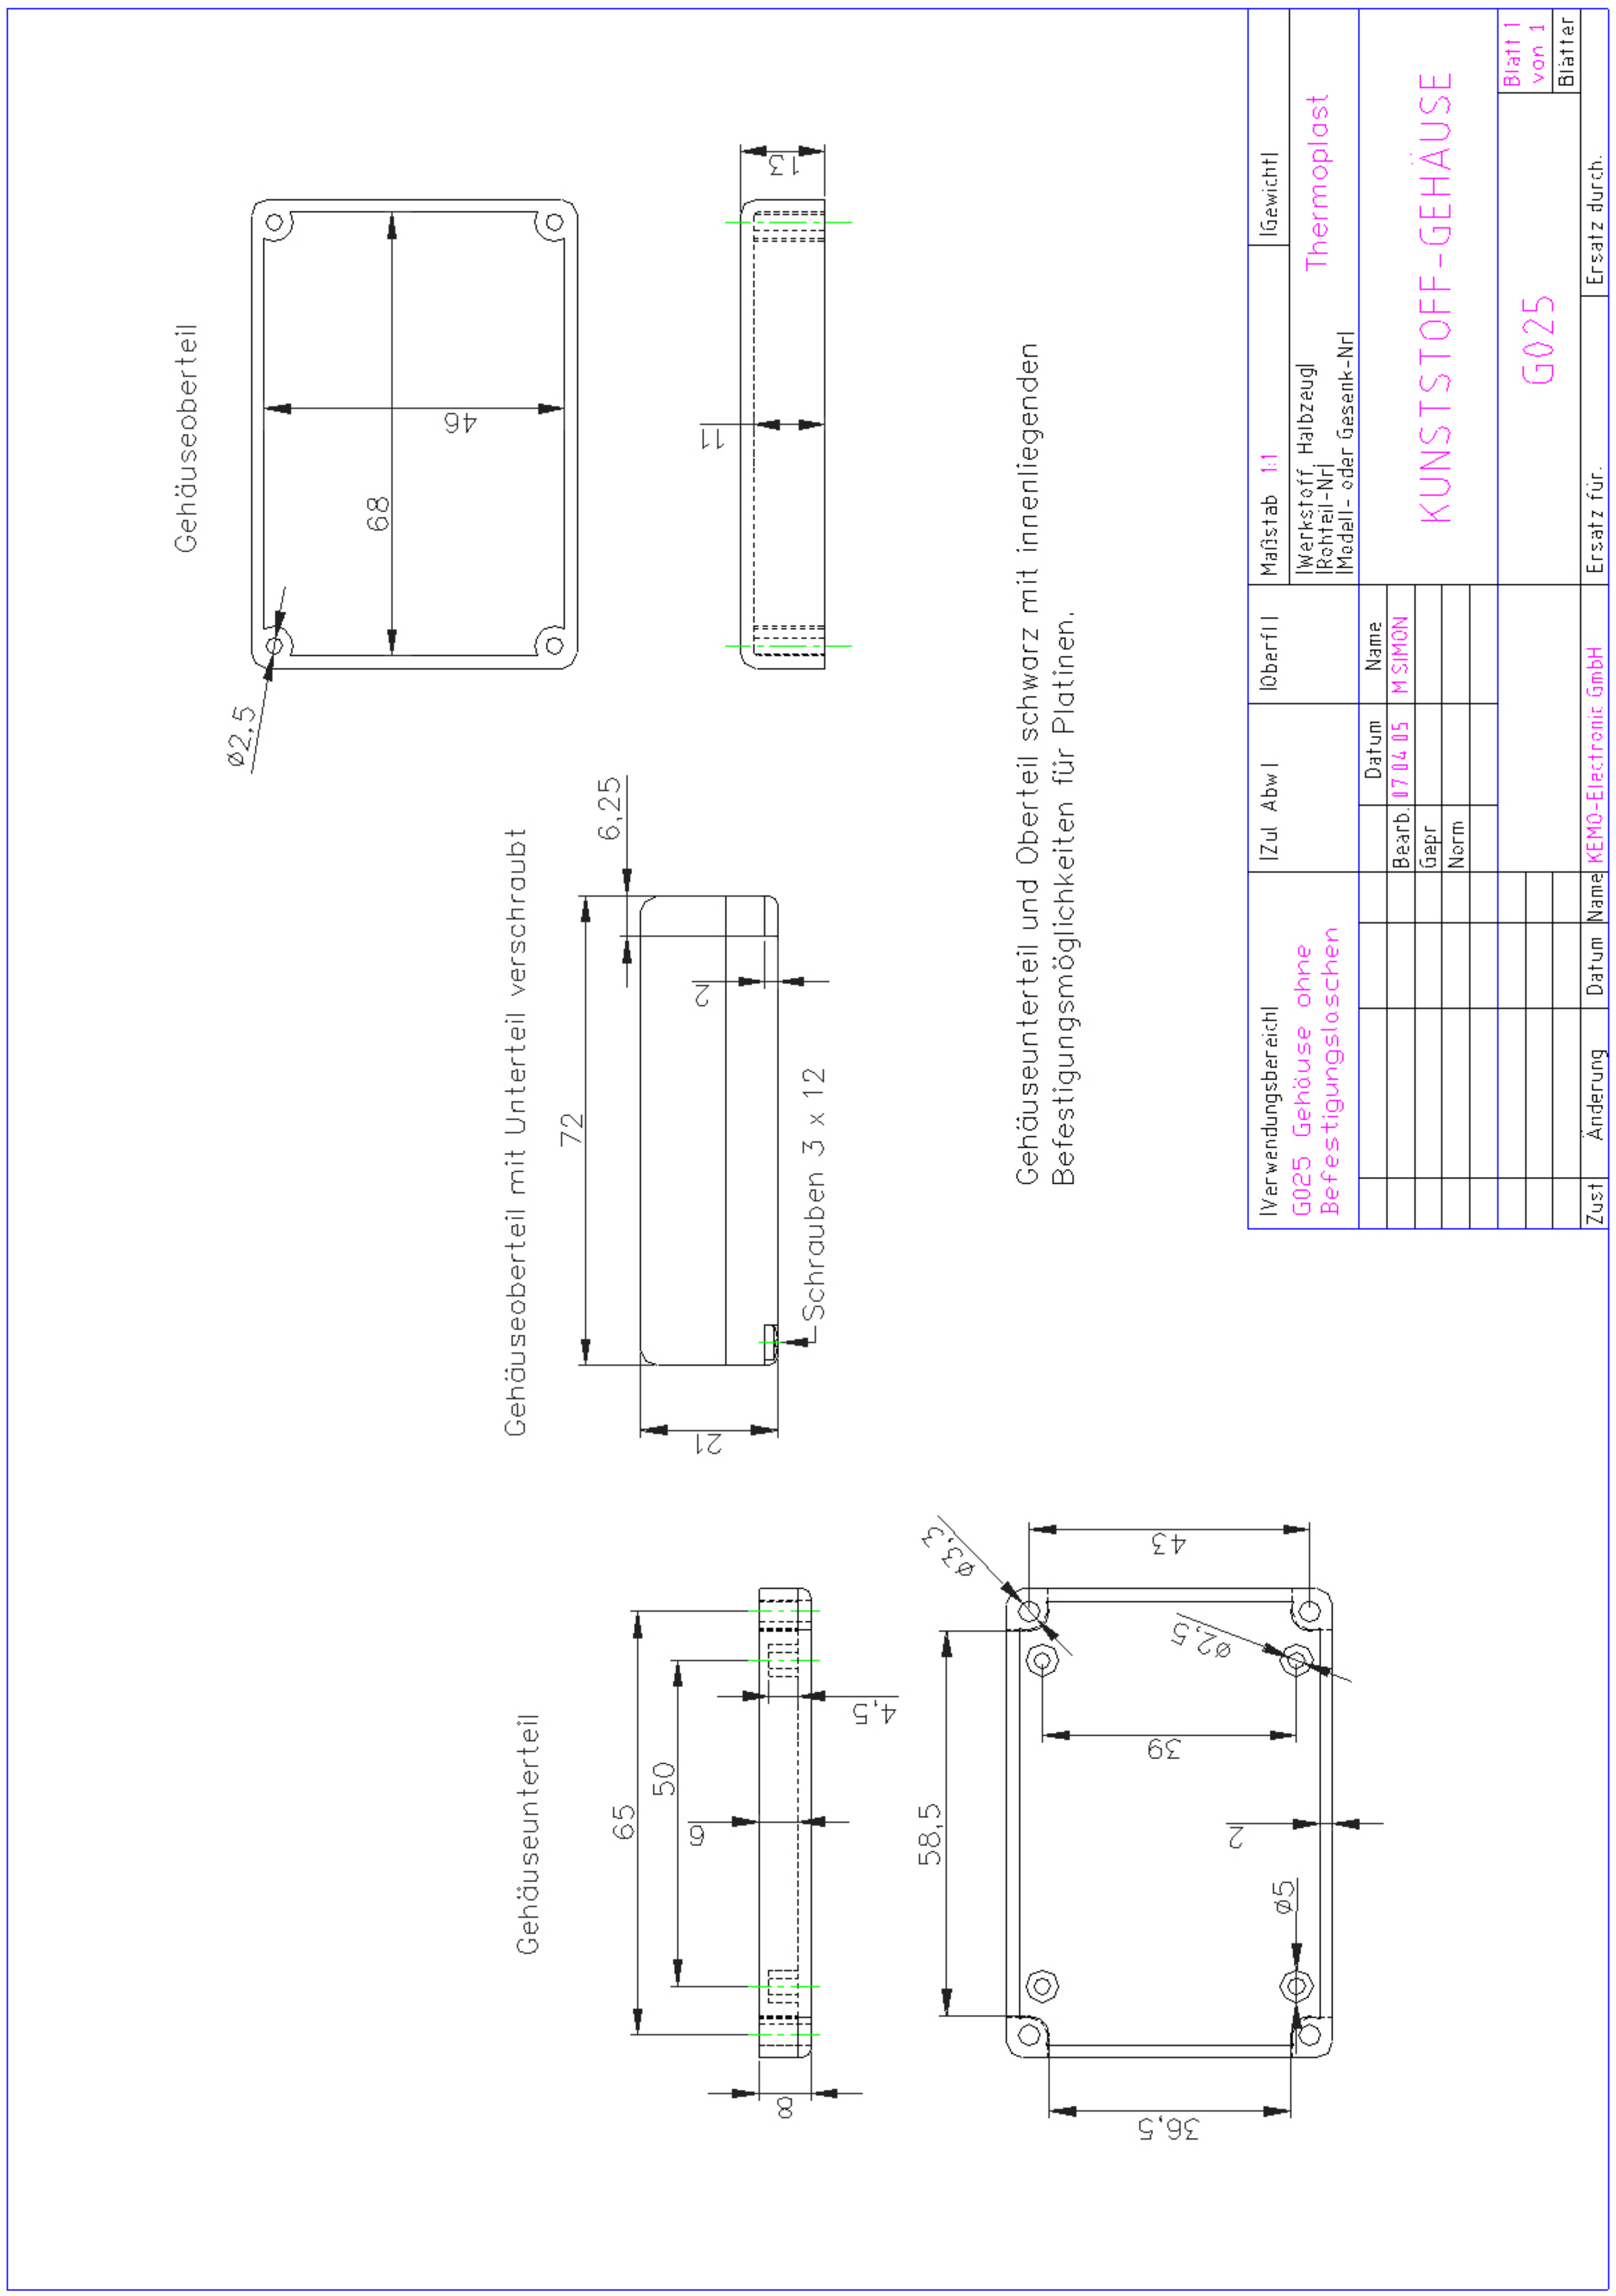
\includegraphics[scale=0.8]{Gehauseplan.png}
\end{center}

\section{Änderungen am Gehäuse}



\end{document}